\chapter{Implementation: DApp}
DApp is frequently characterized as P2P, trustless, with the unique quality that it cannot be controlled by a single server. DApps have at least one user interface or frontend, which could be a desktop program running on a PC or a mobile app.
A single organization or business may give the application's data, or end users may do it directly.
DApp processes and stores data using smart contracts on Ethereum as the backend. DApp user interfaces typically resemble standard websites, but they also include one or more smart contracts \footnote{https://github.com/zahrajoonjafari/MasterThesis/tree/master/ontology-dalicc-connector} \cite{William}.

\begin{center}
	
	\begin{figure}[htb!]
		
		\begin{minipage}{0.75\linewidth}
			
			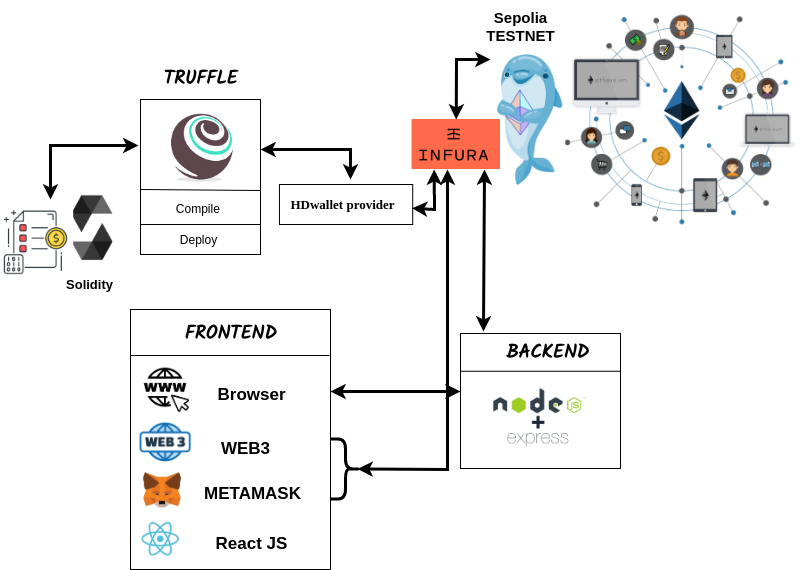
\includegraphics[width=1.45\textwidth]{images/chap03_dapp.png}
		\end{minipage}
		\caption{DApp infrastructure}
		
	\end{figure}
	
\end{center}

\section{Ethereum DApp}
The benefits of using the Ethereum blockchain in DApps are as follows \cite{William}:
\begin{itemize}
    \item 1- The user can see what is going on before submitting any data.
    \item 2- Once the user has interacted, no one can tamper or delete data.
    \item 3- The user of the application can directly participate in application management.
\end{itemize}
\section{Project Concepts}

In this section, we focused on the requirements that we need to address in our application.
\\
\subsection{Contract and Ontology Specification}
Here, we explain some terms related to smart contracts and the ontology of our application. These are needed as the primary requirement to build up this dApp.
\begin{itemize}
\item \textbf{Definition 1 (Owner)} is the address of a deployed contract or transaction on the blockchain. This is the first person who interacts with the contract. In this case, the owner can change the license of the file.\\
	\item \textbf{Definition 2 (Non-owner)} is another user that makes no action. In this case, they can retrieve license information related to specific files.\\
	\item \textbf{Definition 3 (Licensor)} is the address currently interacting with the smart contract. In this case, they can license their file.\\ 
	\item \textbf{Definition 4 (Semantic mappings)}: As we do not have the authority to change stored data on the Ethereum blockchain, one idea is to create a template to have a semantic view of the blockchain.
	To reach this purpose, we need a mapping between stored transaction data in the blockchain and transaction concepts defined as an ontology, then make a query on the produced data from this mapping. This process consists of three following requirements:
	
	\begin{itemize}
		\item \textit{Transaction Schema} are actually some attributes resulting from web3.eth functions that EthOn data properties would be mapped to.
		\item \textit{Transaction Triple template} defines the relationship between concepts (block or transaction) and properties. It is known as 'Subject predicts Object' where the Subject is the web3.eth properties, predict is the EthOn ontology predictor (data properties) and Object (web3.eth properties) is a place that would be replaced by the transaction schema on the mapping. 
		\item \textit{Triplize} is the function that generates data in RDF format by creating a mapping between the two parameters mentioned above as input.
	\end{itemize} 
     \item \textbf{Definition 5 (Prefix)} Name is the label or local part separated with ':' and is the abbreviation of terms that reference resources explicitly. According to Wikipedia, Prefixes are declared at the top of the SPARQL query and our triple template, so that the statements can refer to.\\
     \textbf{Definition 6 (Triple)} Defined in Wikipedia as a statement with three entities that codifies semantic data in the form of \textit{Subject-predicate-Object} expressions.\\
\end{itemize}
\subsection{Technology Usage}
\textbf{DApp\footnote{https://www.techtarget.com/iotagenda/definition/blockchain-dApp}} \\
Based on an internet definition, it is a type of open-source smart contract application that runs on a decentralized peer-to-peer network rather than a centralized server. It allows users to transparently execute a transaction on a distributed network. \\
DApp is similar to centralized apps, as they use frontend and backend. The backend of an app is supported by a centralized server or database, whereas the backend of a DApp runs on a decentralized P2P network and is supported by smart contracts stored on the Ethereum blockchain.\\
\\
\textbf{Decentralized Application Characteristics:}\\
	\textit{Open Source}: All the requirements are decided by consensus of all available users on a network.\\
	\textit{Decentralized Storage}: Data is stored on decentralized blocks.\\
	\textit{Validation}: As the application runs on blockchain, they offer validation of data using cryptographic tokens which are needed for the network. \\
 \\
\textbf{Ethereum} \\
it is explained in section 1.4.\\
\\
\textbf{Solidity} \\
it is explained in section 1.5.5.\\
\\
\textbf{SHA3-256} \\It is explained in section 1.5.3.\\
\\
\textbf{Java Script Tools} 
\begin{itemize}
  \item \texttt{Truffle} is the smart contract development tools and testing network for blockchain applications and supports developers who are looking to build their dApp, etc. \\
   Truffle offers some different features:
 \begin{itemize}
\item\textit{Smart Contract Management}: Truffle helps to manage artifacts of smart contracts used in dApp and supports library linking, deploying, and other Ethereum dApps. \\
 \item\textit{Contract Testing System}: Truffle helps developers construct smart contract testing systems for all their contracts. \\
 \item\textit{Network Management} helps developers by managing their artifacts. \\
 \item\textit{Truffle Console} allows the developer to access all Truffle commands and build contracts \footnote{https://moralis.io/truffle-explained-what-is-the-truffle-suite}.
 \end{itemize}

\item \texttt{React.js} is an open-source JavaScript framework which is used as a frontend. In React, a developer builds a web application by using reusable individual components that are assembled from an application's whole user interface.\\
React has the advantage of providing a feature that combines the speed of JavaScript with a more efficient method of managing DOM to render web pages faster and create more responsive web applications.\footnote{https://blog.hubspot.com/website/react-js}.\\
\item \texttt{crypto.js} is the JavaScript library that performs data encryption and decryption. It is a collection of standard algorithms including SHA3-256 \footnote{{https://github.com/jakubzapletal/crypto-js}}.
\item \texttt{Web3.js} helps developers to connect to the Ethereum blockchain. It is a collection of libraries that allows developers to perform such actions as sending ether, checking data from smart contracts, and creating smart contracts \footnote{https://www.datastax.com/guides/what-is-web3.js}.\\
\item \texttt{axios} provides HTTP requests from the browser and handles request/response data \footnote{https://axios-http.com/docs/intro}.\\
\item \texttt{HDWalletProvider} is a package that helps developers to connect to a network by configuring the connection to the Ethereum blockchain through \textit{Infura}. This provider is used by Truffle when deploying contracts. In addition, MetaMask providers are also used when we want to interact with the contract in the browser. 

HDWalletProvider provides a custom URL: 'http://127.0.0.1:7545'. This will spawn a development blockchain locally on port 7545 \footnote{https://github.com/trufflesuite/truffle-hdwallet-provider}. \\
\item \texttt{Express.js} is a Node.js framework for developing dApps. It provides HTTP methods (GET, POST) to call functions for particular URL routes \footnote{https://www.simplilearn.com/tutorials/nodejs-tutorial/what-is-express-js}. \\ 
When we run a dApp, we have an HTTP server located on port 3000. \\
\item \texttt{FS} provides some functionality to interact with the file system, mostly used functions like: \textit{readFileSync}, \textit{writeFileSync} and \textit{appendFileSync} \footnote{https://blog.risingstack.com/fs-module-in-node-js/}. \\
\end{itemize}

\textbf{Semantic Web Tools}\\
\begin{itemize}
	\item \textit{EthOn Ontology} is a semantic view of the Ethereum blockchain. It encompasses different classes and relations to cover different concepts of Ethereum such as blocks, transactions, and messages to formalize RDF triples. We used classes and properties related to transaction concepts as a template to model our transaction to DALICC \footnote{https://axios-http.com/docs/intro}.
	\item \textit{SPARQL query} is defined in Section 2.1.4.
	\item \textit{Command-Line SPARQL} is a utility of Apache Jena that runs queries on remote SPARQL endpoints or RDF files located on a local computer or web. We used the command as follows \footnote{http://richard.cyganiak.de/blog/wp-content/uploads/2013/09/jena-sparql-cli-v1.pdf}:\\
	 - Using command line : \textit{sparql --data rdfFile --query sparqlFile}
\end{itemize}
\textbf{Ethereum Tools}

\begin{itemize}
\item \textit{Infura} is a web3 backend and infrastructure-as-a-Service (IaaS) provider that offers a range of tools to help developers build dApps to connect to the Ethereum blockchain \footnote{https://blog.infura.io/post/getting-started-with-infura-28e41844cc89}.\\
\item \textit{Metamask} is a wallet used to interact with the Ethereum blockchain. It allows users to connect to the network through a browser extension or mobile app. Metamask wallet stores all accounts, each account having its own private key \footnote{https://originstamp.com/blog/metamask-what-is-it-and-how-does-it-work/}.\\
\item \textit{Faucet (ETH faucet)} is the platform that gives some test tokens to a user to test smart contracts or send transactions before deploying them to the mainnet \footnote{https://changelly.com/blog/best-ethereum-faucets/}. \\
\item \textit{Testnets} are the test blockchain networks that behave similarly to the main blockchain (mainnet). This allows developers to execute their contracts on the test blockchain freely before executing on the main network \footnote{https://blog.infura.io/post/introducing-infuras-eth-testnet-faucet-get-0-5-eth-daily-to-test-your-dapps}. \\
Infura's new testnet faucet is Sepolia ETH which provides the most reliable and high-volume faucets for developers.\\
\item \textit{Web3.eth} is a package that allows interacting with the Ethereum blockchain. It contains many functions to provide more information about executed smart contracts or transactions on the blockchain \footnote{https://web3js.readthedocs.io/en/v1.2.11/web3-eth.html}. 
In our case, some functions including: \textit{getBlock}, \textit{getTransaction} and \textit{getTransactionReceipt} are chosen to provide some more details which are mapped to EthOn ontology objects properties. These retrieved properties would be used later in triples.\\
\item \textit{Knowledge graph} indicates classes and relations.
The idea is to use a graph-based data model to clarify survived transactions, their classes, and relations in much more detail.
\begin{center}
	
	\begin{figure}[htb!]
		
		\begin{minipage}{0.75\linewidth}
			
			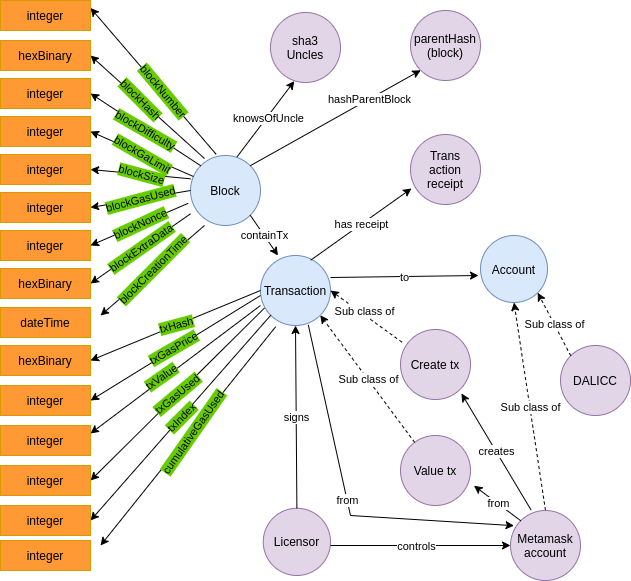
\includegraphics[width=1.45\textwidth]{images/chap03_knowledge_graph.png}
		\end{minipage}
		\caption{Transaction illustration}
		
	\end{figure}
	
\end{center}

\end{itemize}
\section{Project Architecture}

\subsection{Backend} The backend of this project relies on the Ethereum platform using smart contracts. In addition, DALICC license library the user can license their data or retrieve license information. In the next paragraph, we will focus more on authenticated users as the main challenge in decentralized apps and data licensing systems by users.\\
\\
\textbf{Authenticated user \footnote{https://medium.com/coinmonks/how-to-do-authentication-in-decentralized-application-dapp-d9bc66b6249c}} \\
\\
Authentication of users on Ethereum for validation purposes is an essential feature when building dApps. Therefore, programming the functionality of Ethereum authentication for dApps is important for blockchain developers. 
In this dApp, we consider two solutions for Ethereum authentication as follows: \\
\\
\textit{- log in to MetaMask:} MetaMask is the most popular cryptocurrency wallet (Ethereum account) to support the Ethereum blockchain. Additionally, MetaMask is a bridge for web3 authentication to an Ethereum-based decentralized application. By logging into MetaMask, users can submit transactions or check the stored data on the blockchain.\\
\\
\textit{- Using Smart Contract:} The address of the MetaMask is passed to the smart contract as a licensor, then it will use this address as an owner to license their file. \\
\\
\textbf{Licensing in Smart Contract} follows: \\
\\
\textbf{License Information}: It represents three elements: licensor address that is passed by MetaMask, the license of the data, and the URI related to this license.\\
\textbf{Storage License Information}: \\Each smart contract that runs on the Ethereum blockchain would be maintained in its permanent storage. The license information is stored in its storage and is changeable only by the smart contract itself.\\
\textbf{Retrieve License Information}: \\As mentioned earlier, only a smart contract can change the data in its memory. Thus, we can consider smart contract as a validating system for license requests. The JavaScript library web3.js is an interface to the Ethereum network for the frontend of this dApp. This allows the frontend to access the smart contract, retrieving or changing license information.\\
\subsection{Frontend}
Frontend of this project built with React.js, HTML, and CSS. The React.js is used in this frontend to create the user interface.\\
\\
\textbf{User Roadmap}\\
The licensing data from the user interface goes through three phases:
\begin{itemize}
	\item The user is asked to select a license type from the DALICC Library via Axios and make a request in the frontend. Then, after selecting data in the next field, the user should check if the selected file is already licensed or not. Depending on this verification, the user receives either the confirmation message 'License Detected' or the rejection message 'License Not Detected'.
   \item The user should go further by pressing the 'License Data/Retrieve License' button to get license information for the confirmation message of the last phase or license their file.\\
    License information contains some information like license type, license URI retrieved from the DALICC library, and the address of the owner of this license. For licensing data, the user is asked to log in to MetaMask for the authentication process and this address is passed to the smart contract as owner of this license. The licensing process is done by receiving the hash value of the licensed data.
   \item In the last phase, the user can observe the receipt of this transaction in a table that contains transaction details from the interaction between \textit{web3.eth} and \textit{ethOn} ontology.
 \end{itemize}
 \begin{center}
 	
 	\begin{figure}[htb!]
 		
 		\begin{minipage}{0.75\linewidth}
 			
 			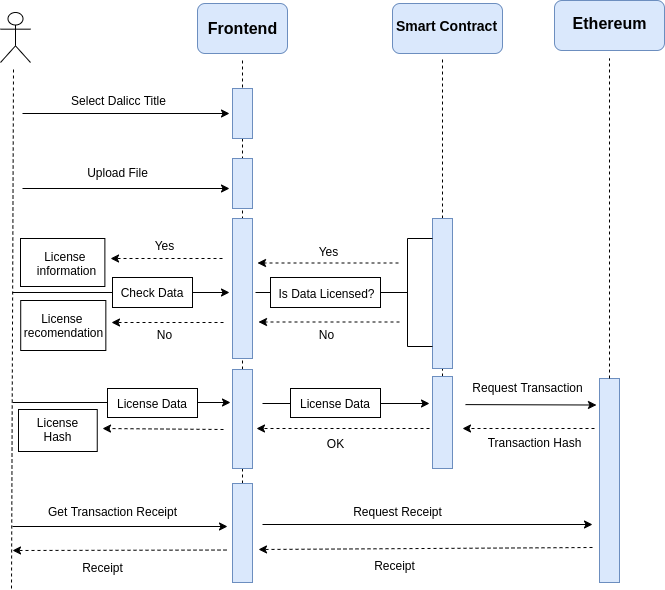
\includegraphics[width=1.45\textwidth]{images/chap03_user_roadmap.png}
 		\end{minipage}
 		\caption{Sequence diagram for licensing file}
  	\end{figure}
  \end{center}
  \textbf{Interaction with Backend}\\
  Since the backend code (smart contract) of the dApp is on a decentralized network, we focused on the interaction between the smart contract and the Ethereum network. The communication between the frontend and backend is taken over by JavaScript library \textit{web3.js}.
  For this purpose, web3 provides this connection either with HDWallet-provider to connect to the test network (Ropsten in our case) or Ethereum provider.\\
 \textbf{Interaction with DALICC} \\
To retrieve the license, an HTTP GET request is sent to the DALICC library endpoint and returns the license which encompasses two elements: license title and license URI. The user can choose just the DALICC title as a license, then the URI of the associated title would be stored subsequently in the smart contract for further processing. \\
\\
\textbf{License receipts} \\
After committing a transaction in the blockchain, the user can get transaction details via \textit{web3.eth}, then send transaction details in RDF format to the server to store in a file. The produced Turtle file will be resulted into a readable format and would be returned to the frontend by an HTTP GET request from the frontend.
\\
\subsection{DApp Architecture} 
This application encompasses some components:
\begin{itemize}
	\item User interface
	\item Smart contract to communicate with DALICC library
	\item Ethereum network to support transactions
	\item Transaction receipt
	\item EthOn ontology
	\item SPARQL query    
\end{itemize}
\begin{center}
   \begin{figure}[htb!]
		
		\begin{minipage}{0.75\linewidth}
			
			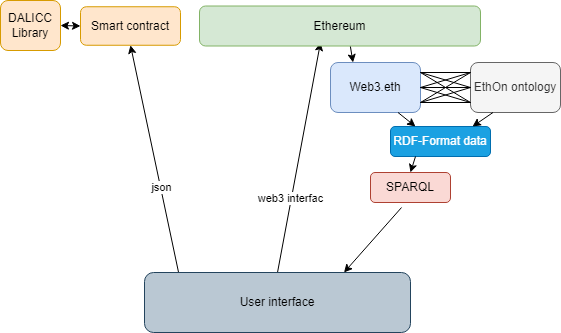
\includegraphics[width=1.5\textwidth]{images/chap03_eth_dalicc_comm.png}
		\end{minipage}
		\caption{DApp architecture}
	\end{figure}
\end{center}

\section{Implementation}
This section comprises the implementation details in a smart contract and some main functions in the application.

\subsection{Smart Contract Logic}
As mentioned before, the backend code of this application is on the Ethereum network. In this section, we will contemplate more on each functionality of the contract in this dApp.
\begin{itemize}
	\item \textit{Owned Contract} \\
	This smart contract contains the function to prevent non-owner users from calling the function. This contract contains a function that helps us to restrict access to some functions in another contract. \\
	\item \textit{PrimaryLicenseContract} \\
	This is the main contract that communicates with two other contracts to represent the public interface of the licensing system. It provides functions to license data or retrieve license information. \\
   \item \textit{LicenseManager Contract} \\
	This smart contract is responsible for saving the address of the license or creating one for the new file. \\
	\item \textit{License Contract} \\
	The hash value and licensor address will be stored in this contract. License contract represents only one license and associated license contract for this license. The license contract should have been created by the license manager.
\end{itemize}

\begin{center}
	
	\begin{figure}[htb!]
		
		\begin{minipage}{0.75\linewidth}
			
			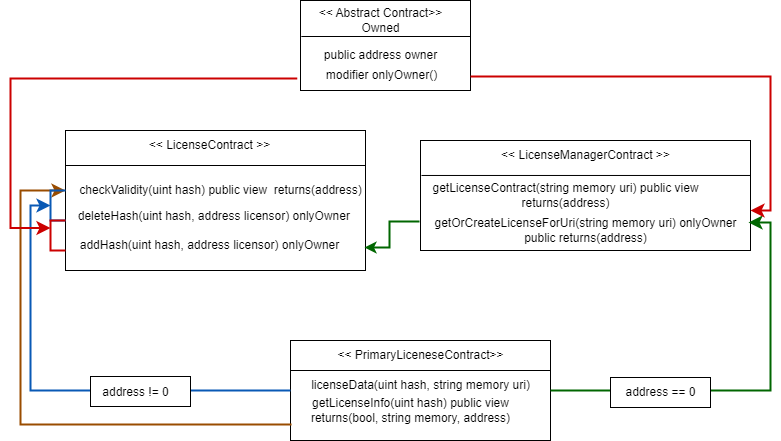
\includegraphics[width=1.45\textwidth]{images/chap03_smartContract_visual.png}
		\end{minipage}
		\caption{Smart contract visualization}
		
	\end{figure}
	
\end{center}

\text{How Does Smart Contract work?}
\begin{itemize}
	\item \textbf{Licensing System Process} \\
    To license data, two parameters are needed. The first one is the hash of related data and the second one is the address related to the URI of the license. This smart contract as a \textit{caller} takes over the process: \\
    \textbf{License Data} \\
    To license data, the function \textit{licenseData} is used which declares two parameters: the first one is the hash associated with selected data, and the second one is the URI of the selected license. By pressing the 'License Data/Retrieve License' on the frontend, the function \textit{licenseData} would be triggered and perform the steps as follows: \\
    This function checks if the target address is the zero account, which means the transaction creates a new contract: 
    if not, the function \textit{deleteHash} is called, otherwise \textit{getOrCreateLicenseForUri} would be called. How does licensing data work? \\
	\begin{itemize}
		\item \textit{licenseData} function checks if the specified hash is linked to a license and the caller is licensor, then \textit{deleteHash} is called and the hash of related data and address of licensor would be passed. \\
		\hspace{1cm} \textbf{Definition} \textit{deleteHash}: This function is accessible only for the owner (function caller), which means the caller of this function must be the owner and the passed address should be the licensor. Then the link between the hash and license will be dropped.
		\item \textit{getOrCreateLicenseForUri} of the license manager is called and the URI of the selected data as input parameter would be passed and returns the address to license contract which represents this URI.\\
		\hspace{1cm}\textbf{Definition} \textit{getOrCreateLicenseForUri}: This function checks if the caller of this function is the owner, then if there exists a license contract for a given URI. If so, the address of this license contract would be returned. Otherwise, a new license contract will be created and the address of the contract will be stored and returned. The caller's address of the caller will also be used later as the owner of this contract.
		\item \textit{addHash} function of the License contract is called with two parameters: the first one is the hash of data, and the second one is the function caller.\\
		\hspace{1cm} \textbf{Definition} \textit{addHash}: This function is accessible only for the owner (function caller), the link between the hash value and the license is created. The second parameter would be stored also as licensor. \\
		\item At the end, the event should be emitted to fire the new changes in \textit{PrimaryLicenseContract}.
		
	\end{itemize}
	\item \textbf{Change License Data} \\
	This is doable just by the licensor in the same way as license data. \\
	\item \textbf{Retrieve License Information} \\
	To retrieve license information, the function \textit{getLicenseInfo} is called, having a hash of data as a parameter, and checks if there is some license information related to this hash. Then, the address is returned; otherwise, a null address and string are returned.
	
\end{itemize}
\subsection{Forntend Workflow}
\begin{itemize}
	\item Define Type:
    In this step, the user is asked to select a license type from among many different licenses. These licenses are loaded from the DALICC License Library via an Axios GET request, and the user must choose one of them to continue the license processing.
 \begin{center}
	\begin{figure}[htb!]
		
		\begin{minipage}{0.45\linewidth}
			\centering
			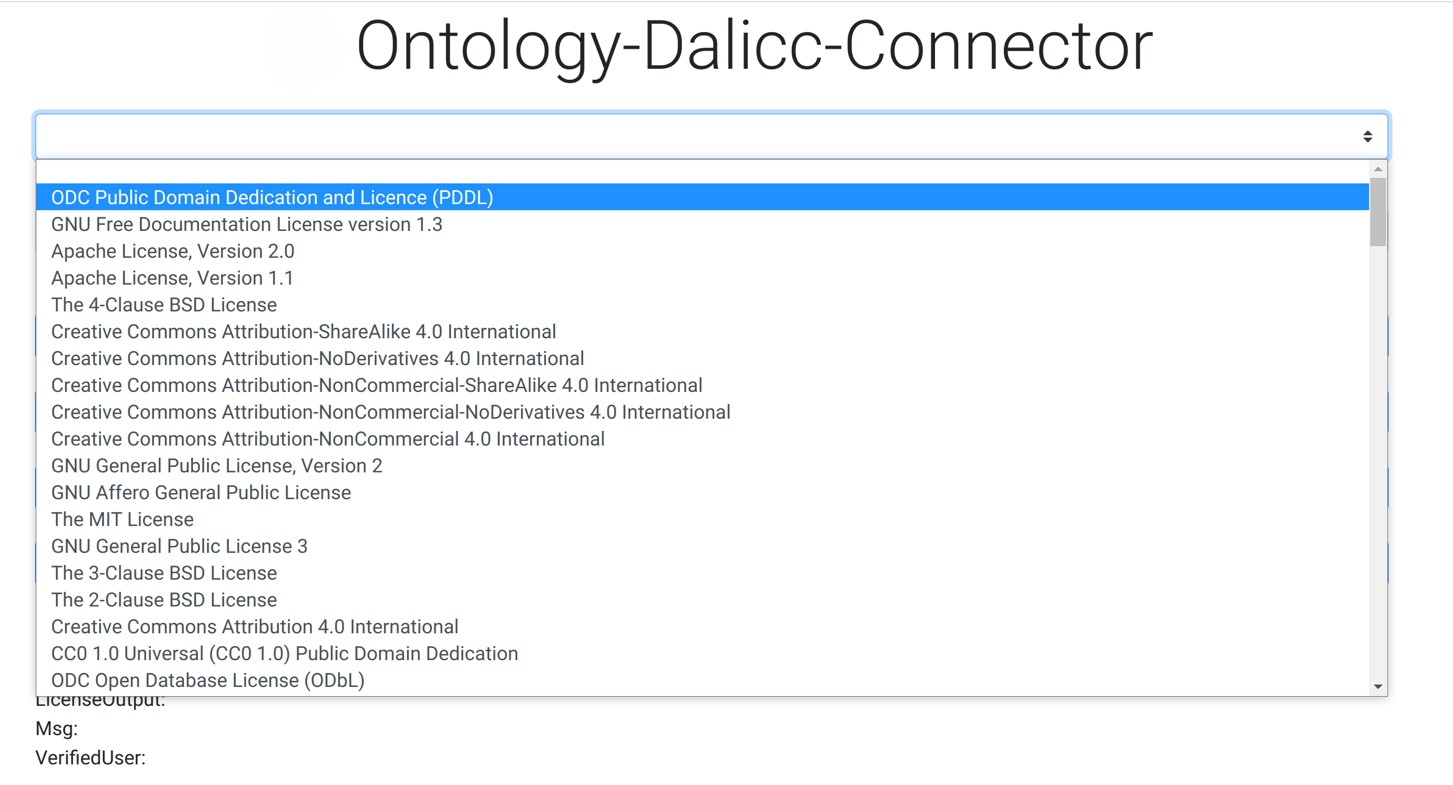
\includegraphics[width=1.95\textwidth]{images/chap03_selectType.jpg}
		\end{minipage}
		\caption[Define type from DALICC library]{Define type from DALICC library}
		
	\end{figure}
	
\end{center}
	\item define content:
    In this step, the user should choose the file or data that they want to license. Subsequently, the hash SHA3-256 of the selected file is calculated, which is used to retrieve license information later.
 \begin{center}
	\begin{figure}[htb!]
		
		\begin{minipage}{0.45\linewidth}
			\centering
			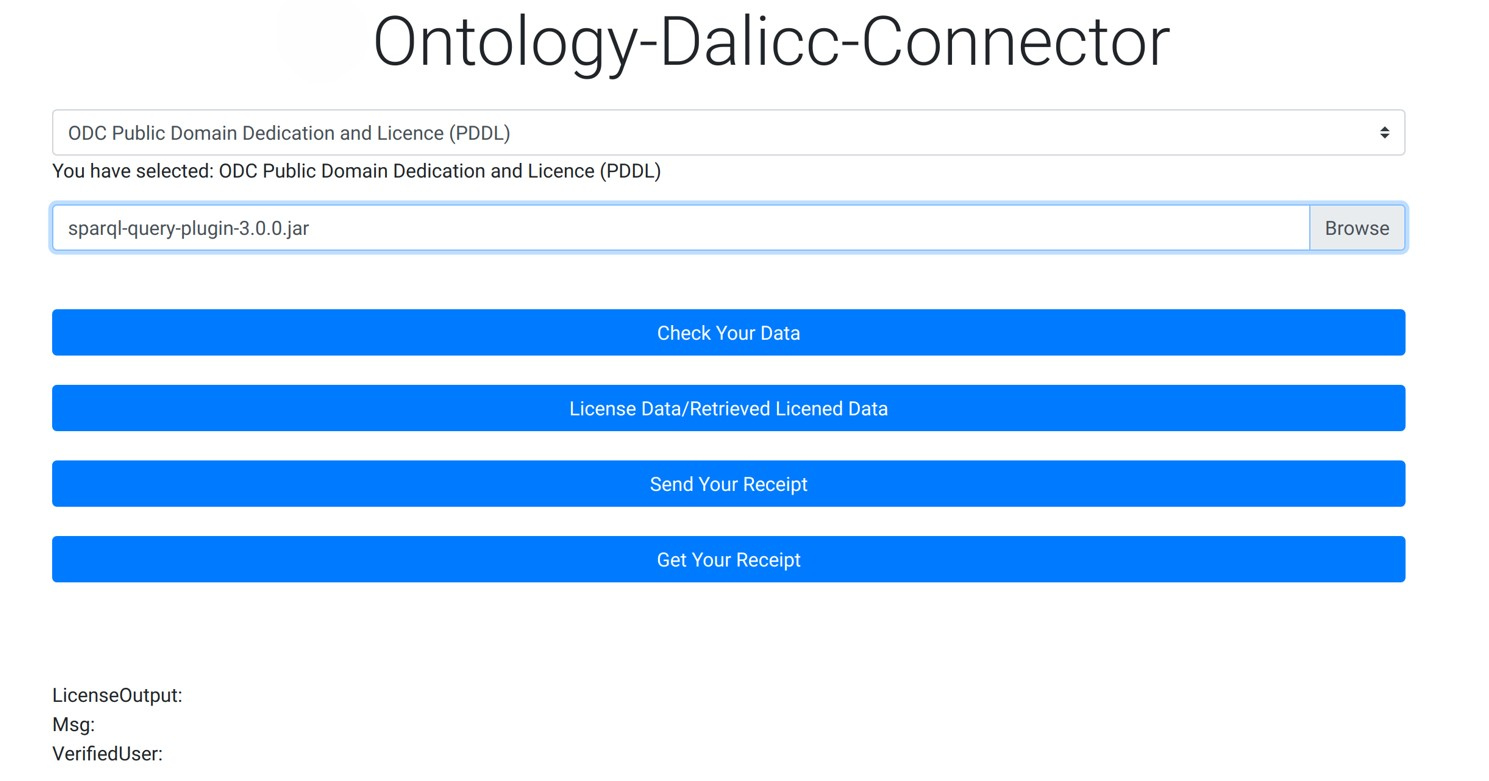
\includegraphics[width=1.95\textwidth]{images/chap03_selectFile.jpg}
		\end{minipage}
		\caption[Define file from local device]{Define file from local device}
		
	\end{figure}
\end{center}
	\item Check Your Data:
	In this step, the user should check the selected data: if it has been licensed before or not. They will receive just a message either confirming 'License is detected' or rejecting 'License is not detected'. They should go further to obtain more information.
    \begin{center}
	\begin{figure}[htb!]
		
		\begin{minipage}{0.45\linewidth}
			\centering
			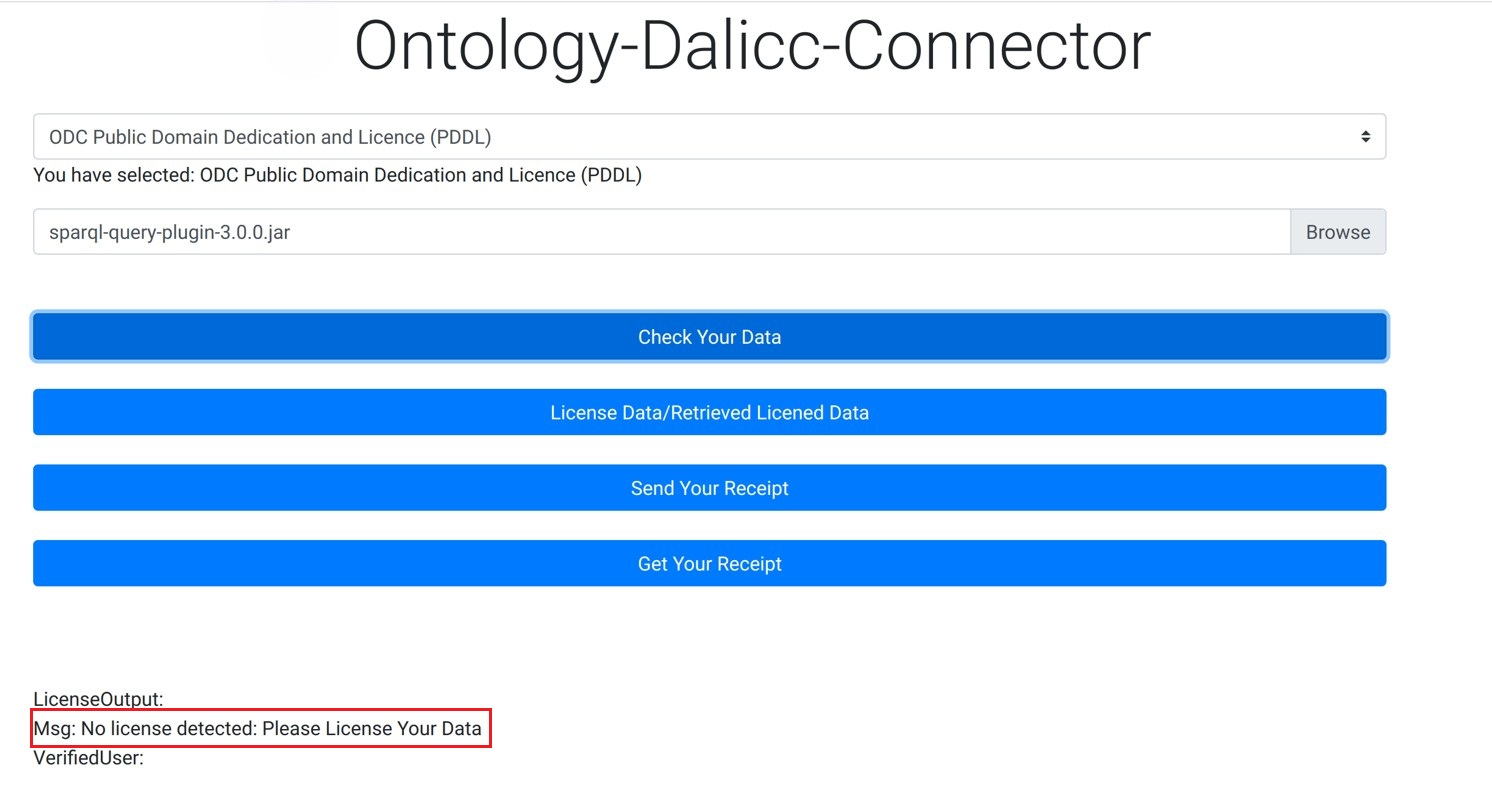
\includegraphics[width=1.95\textwidth]{images/chap03_checkFile.jpg}
		\end{minipage}
		\caption[Check if file is already licensed?]{Check if file is already licensed?}
		
	\end{figure}
	
\end{center}

\begin{center}
	\begin{figure}[htb!]
		
		\begin{minipage}{0.45\linewidth}
			\centering
			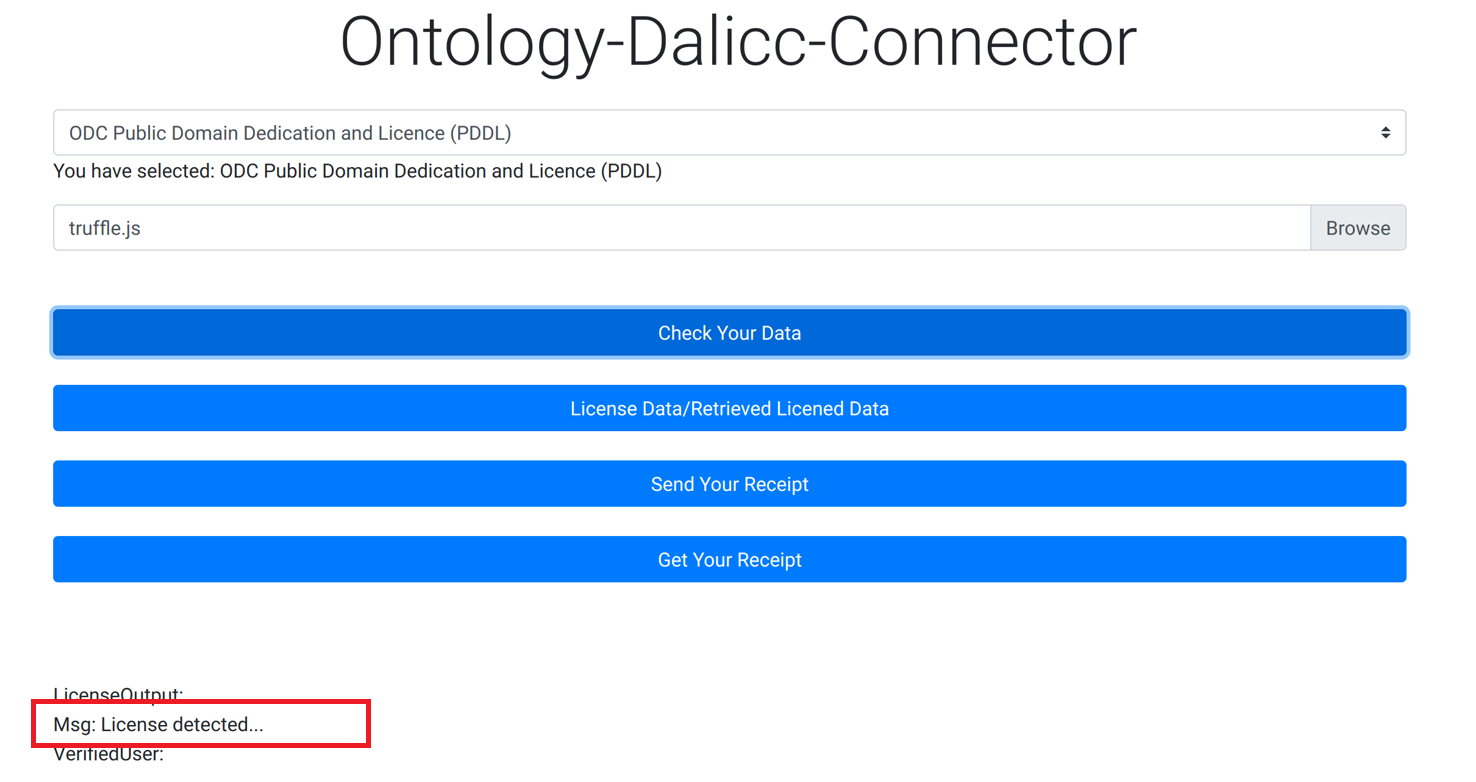
\includegraphics[width=1.95\textwidth]{images/chap03_found_license.png}
		\end{minipage}
		\caption[Message for licensed data]{Message for licensed data}
		
	\end{figure}
	
\end{center}
    \item License Data/Retrieve License Information:
	Here, the user receives the result of that last step, by pressing the hash value of selected data \texttt{SHA3-256} is calculated and passed to the smart contract using \textit{web.js} interface: \\
    \\
	\textbf{-} License information of the selected file or data from which the user received the 'License Detected' message from the last step. The user receives some information related to the license, licensor address, and URI related to the license.\\
    \begin{center}
	\begin{figure}[htb!]
		
		\begin{minipage}{0.55\linewidth}
			\centering
			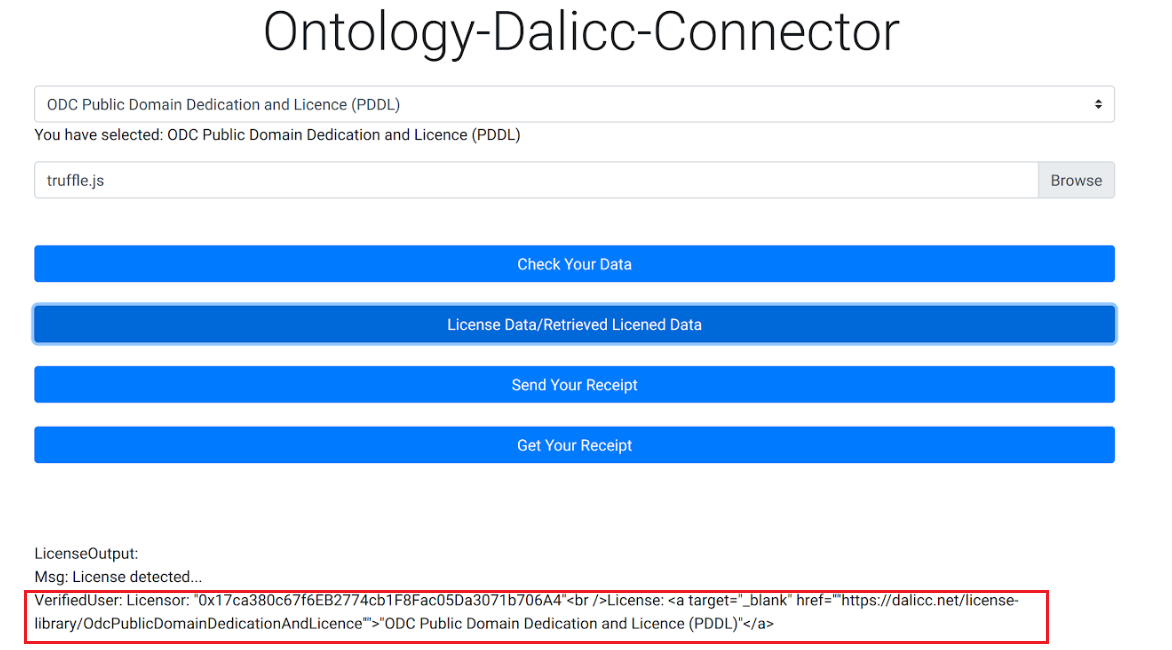
\includegraphics[width=1.95\textwidth]{images/chap03_found_info.png}
		\end{minipage}
		\caption[License information for licensed data]{License information for licensed data}
		
	\end{figure}
	
\end{center}
   \textbf{- } Start licensing his/her file, if they received 'No license detected' from the last step. To license data, the user is asked to log into MetaMask to pass this account as the address of the licensor to the smart contract. The SHA3-256 hash value is calculated and passed by the contract to the Web3 JavaScript interface. Users can see this hash in the frontend, depending on the successful transaction or they receive the error message for failed transaction on the front end.\\
    \begin{center}
	 \begin{figure}[htb!]
		\begin{minipage}{0.45\linewidth}
			\centering
			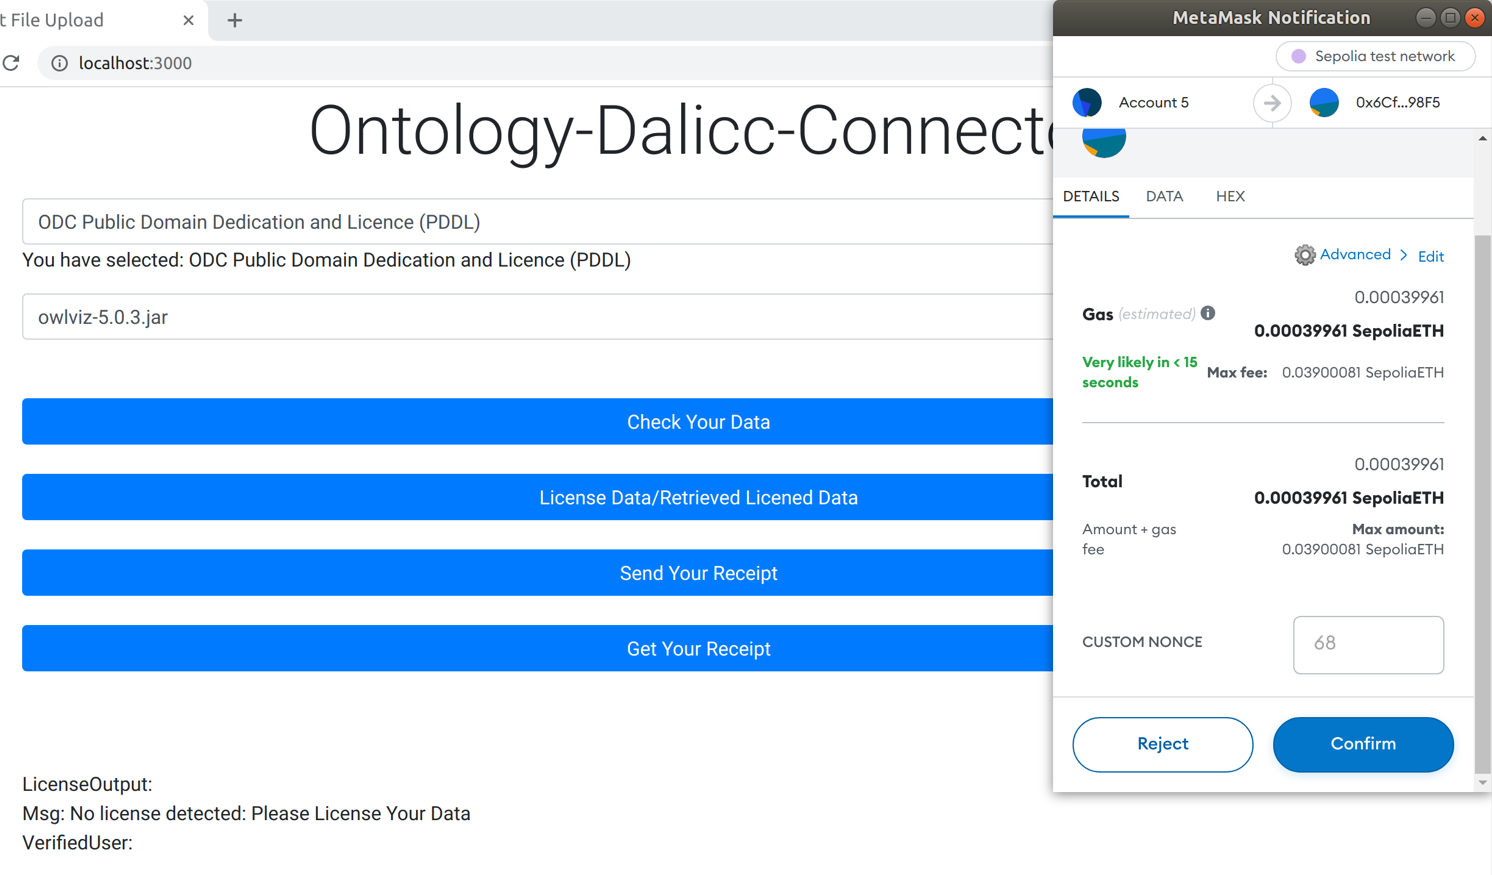
\includegraphics[width=1.95\textwidth]{images/chap03_license_data.png}
		\end{minipage}
		\caption[Licensing data process]{Licensing data process}
		
	\end{figure}
\end{center}
   \begin{center}
	\begin{figure}[htb!]
		
		\begin{minipage}{0.45\linewidth}
			\centering
			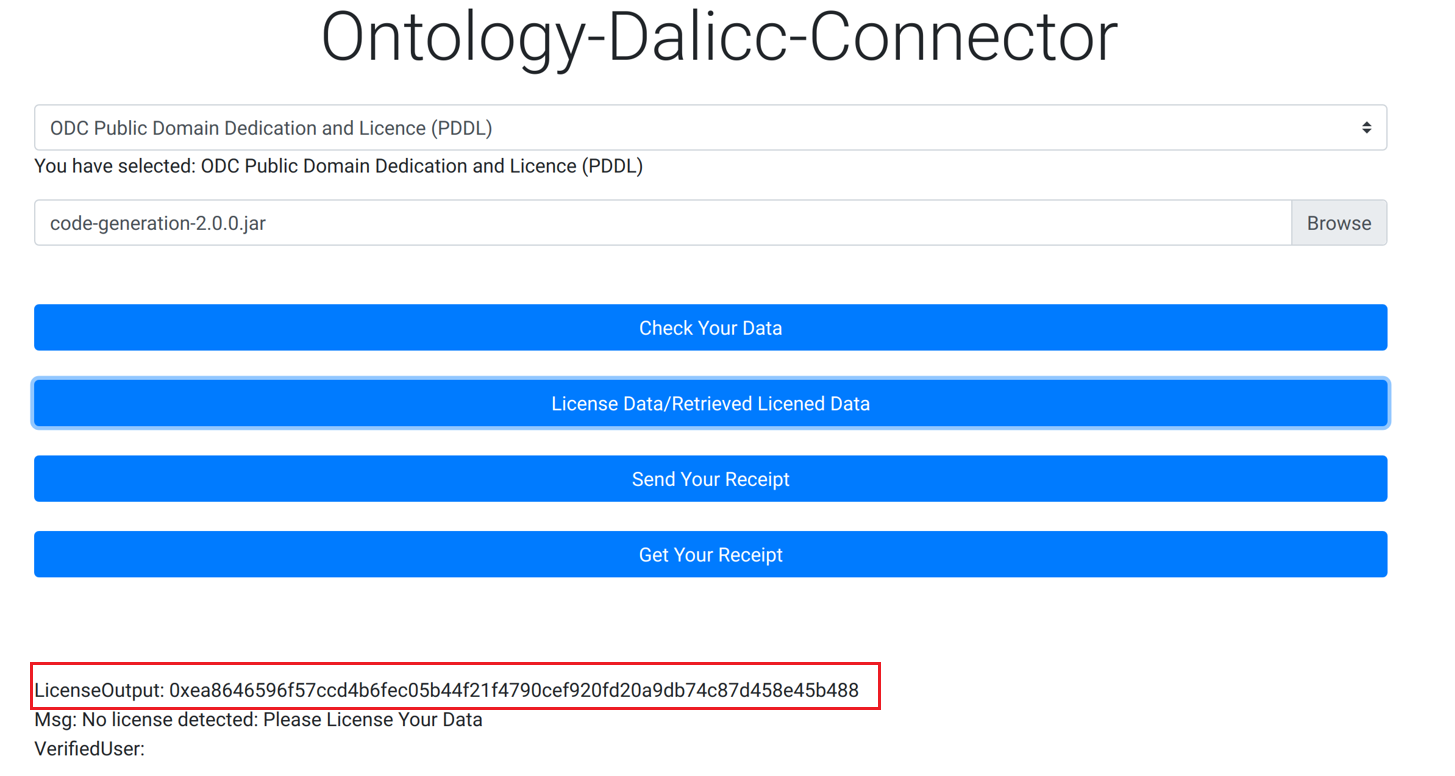
\includegraphics[width=1.95\textwidth]{images/chap03_license_hash.png}
		\end{minipage}
		\caption[License hash after confirming transaction]{License hash after confirming transaction}
		
	\end{figure}
\end{center}
   

\begin{center}
	\begin{figure}[htb!]
		
		\begin{minipage}{0.45\linewidth}
			\centering
			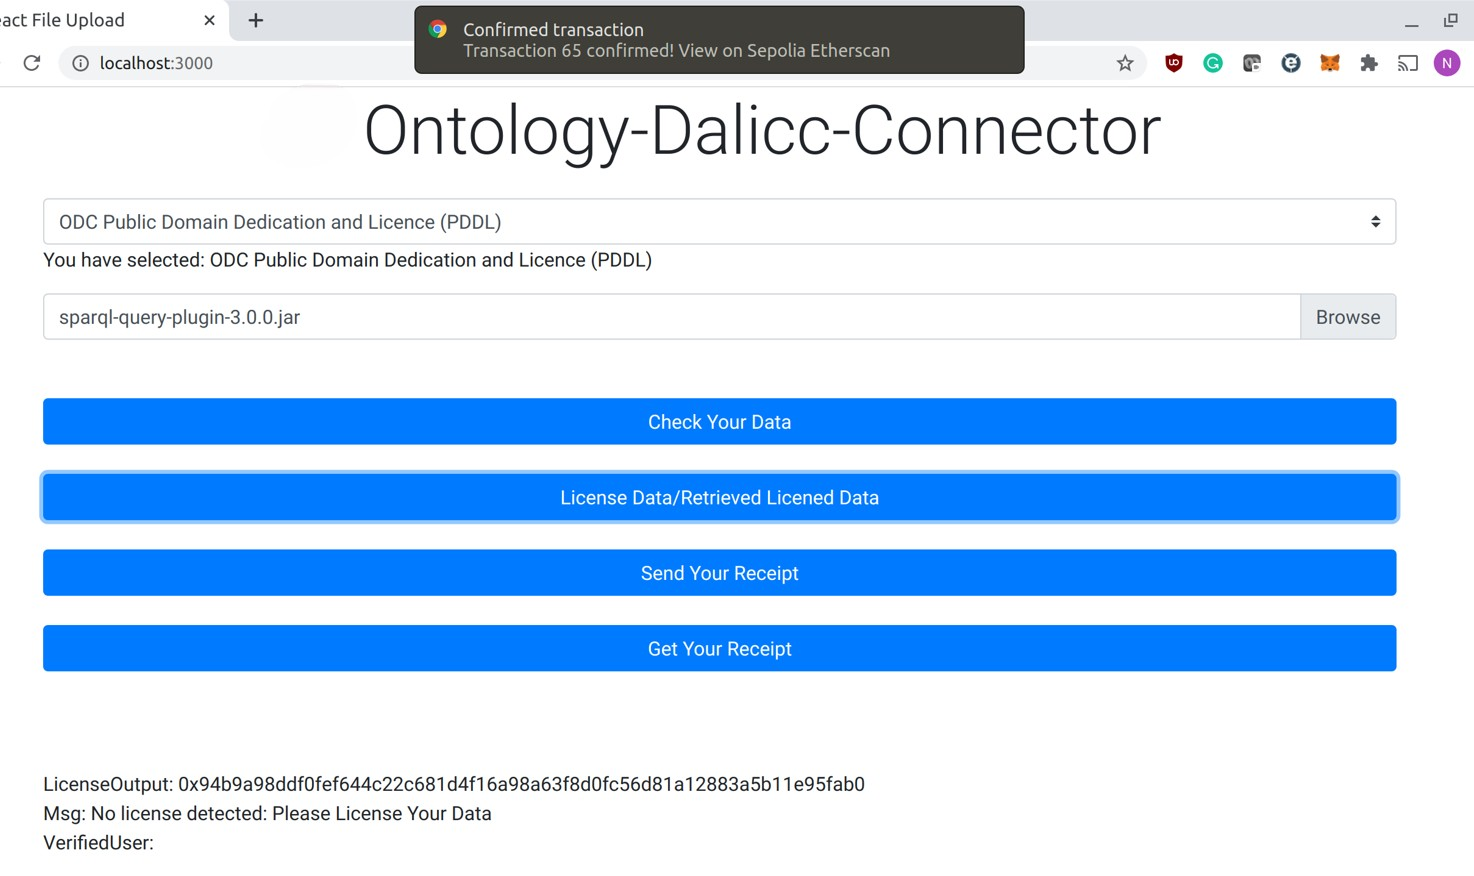
\includegraphics[width=1.95\textwidth]{images/chap03_confirm_tx.jpg}
		\end{minipage}
		\caption[Transaction confirmation]{Transaction confirmation}
		
	\end{figure}
	
\end{center}
	\item Send Transaction: After receiving the hash of the transaction in the frontend, the user goes further to get a receipt of this licensing having all details about the transaction. To have this receipt, the user sends a transaction receipt that is not readable to the server for more processing on this raw result, converting to RDF format data and making a query to produce more readable RDF-based data.
   \item Get Transaction Receipt: In the last step, the user can get a receipt of all transactions that have been done until now as a table.
\end{itemize}

\begin{center}
	\begin{figure}[htb!]
		
		\begin{minipage}{0.55\linewidth}
			\centering
			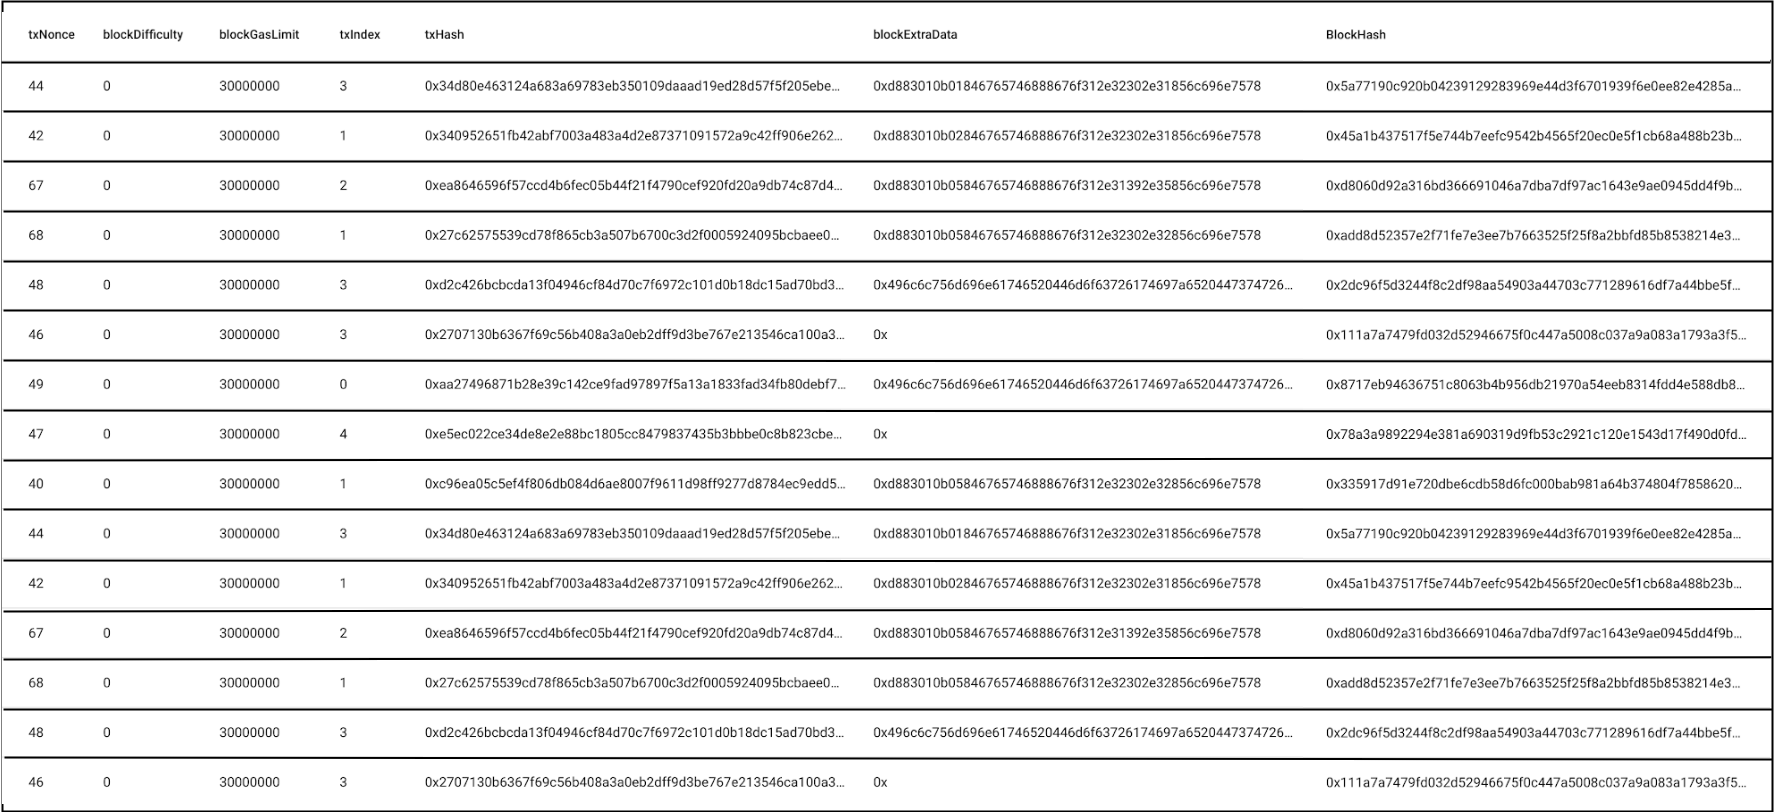
\includegraphics[width=1.95\textwidth]{images/chap03_licese_result_1.png}
		\end{minipage}
		\caption[Result of semantic mapping]{Result of semantic mapping}
		
	\end{figure}
	
\end{center}
\begin{center}
	\begin{figure}[htb!]
		
		\begin{minipage}{0.55\linewidth}
			\centering
			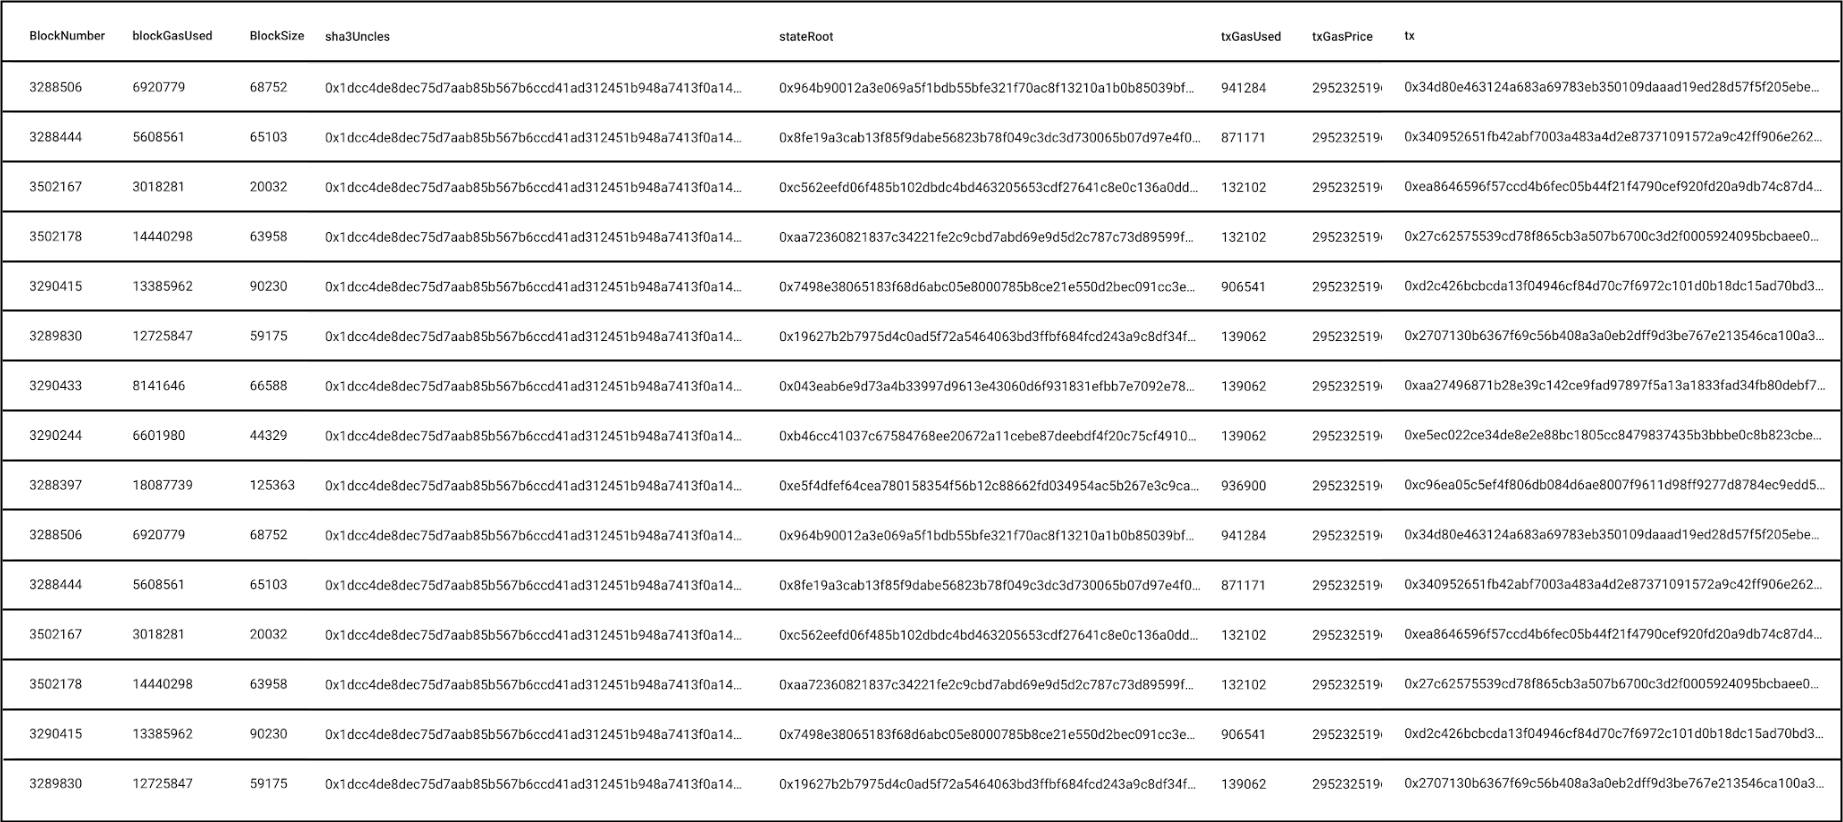
\includegraphics[width=1.95\textwidth]{images/chap03_licese_result_2.png}
		\end{minipage}
		\caption[Result of semantic mapping]{Result of semantic mapping}
		
	\end{figure}
	
\end{center}
